\documentclass[12pt,a4paper]{article}
\usepackage{amsmath,amscd,amsbsy,amssymb,latexsym,url,bm,amsthm}
\usepackage{epsfig,graphicx,subfigure}
\usepackage{enumitem,balance}
\usepackage{wrapfig}
\usepackage{mathrsfs,euscript}
\usepackage[usenames]{xcolor}
\usepackage{hyperref}
\usepackage[vlined,ruled,linesnumbered]{algorithm2e}
\hypersetup{colorlinks=true,linkcolor=black}

\newtheorem{theorem}{Theorem}
\newtheorem{lemma}[theorem]{Lemma}
\newtheorem{proposition}[theorem]{Proposition}
\newtheorem{corollary}[theorem]{Corollary}
\newtheorem{exercise}{Exercise}
\newtheorem*{solution}{Solution}
\newtheorem{definition}{Definition}
\theoremstyle{definition}

\renewcommand{\thefootnote}{\fnsymbol{footnote}}

\newcommand{\postscript}[2]
 {\setlength{\epsfxsize}{#2\hsize}
  \centerline{\epsfbox{#1}}}

\renewcommand{\baselinestretch}{1.0}

\setlength{\oddsidemargin}{-0.365in}
\setlength{\evensidemargin}{-0.365in}
\setlength{\topmargin}{-0.3in}
\setlength{\headheight}{0in}
\setlength{\headsep}{0in}
\setlength{\textheight}{10.1in}
\setlength{\textwidth}{7in}
\makeatletter \renewenvironment{proof}[1][Proof] {\par\pushQED{\qed}\normalfont\topsep6\p@\@plus6\p@\relax\trivlist\item[\hskip\labelsep\bfseries#1\@addpunct{.}]\ignorespaces}{\popQED\endtrivlist\@endpefalse} \makeatother
\makeatletter
\renewenvironment{solution}[1][Solution] {\par\pushQED{\qed}\normalfont\topsep6\p@\@plus6\p@\relax\trivlist\item[\hskip\labelsep\bfseries#1\@addpunct{.}]\ignorespaces}{\popQED\endtrivlist\@endpefalse} \makeatother

\begin{document}

\noindent

%========================================================================
\noindent\framebox[\linewidth]{\shortstack[c]{
\Large{\textbf{Lab08-Graph Exploration}}\vspace{1mm}\\
CS214-Algorithm and Complexity, Xiaofeng Gao, Spring 2020.}}
\begin{center}
\footnotesize{\color{red}$*$ If there is any problem, please contact TA Yiming Liu.}

% Please write down your name, student id and email.
\footnotesize{\color{blue}$*$ Name: Yulong Hui  \quad Student ID: 518030910059 \quad Email: qinchuanhuiyulong@sjtu.edu.cn }
\end{center}

\begin{enumerate}
    \item
    \textbf{BFS Tree.} Similar to DFS, BFS yields a tree, (also possibly forest, but \textbf{just consider a tree} in this question) and we can define \textbf{tree, forward, back, cross} edges for BFS. Denote $Dist(u)$ as the distance between node $u$ and the source node in the BFS tree. Please prove:
    \begin{enumerate}
    	\item For both undirected and directed graphs, no forward edges exist in the graph.
    	
    	\item There are no back edges in undirected graph, while in directed graph each back edge $(u,v)$ yields $0\leq Dist(v)\leq Dist(u)$.
    	
    	\item For undirected graph, each cross edge $(u,v)$ yields $|Dist(v)-Dist(u)|\le 1$, while for directed graph, each cross edge $(u,v)$ yields $Dist(v)\leq Dist(u)+1$.
    	
    \end{enumerate}

~\\
   \textbf{Solution.}
   
   \begin{enumerate}
 	\item We can prove it by contradiction. 
 	
 	Assume that there exists a forward edge $(u,v)$ in a graph (either undirected or directed), which means vertex $v$ is a descendant and is processed later. When we get to process the vertex $u$, edge $(u,v)$ means we can directly get access to $v$ at the next layer. That's to say, we will get a tree edge not a forward edge, because $v$ is just a child of $u$.
 	
 	Then, this is contradictory to the assumption, so no forward edges exist in the graph.
 	
 	\item First, we will talk about the undirected graph by contradiction (similar to question(a) ).
 	
 	Assume that there exists a back edge $(u,v)$ in an undirected graph,which means vertex $u$ is a descendant and is processed later. When we get to process the vertex $v$, edge $(u,v)$ means we can directly get access to $u$ at the next layer. That's to say, we will get a tree edge not a back edge, because $u$ is just a child of $v$.
 	
 	Therefore,  this is contradictory to the assumption, so no back edges exist in the undirected graph.
 	
 	Next, we will talk about the directed graph.
 	
 	The back edge is expressed as $(u,v)$, which means $v$ is an ancestor of $u$ in the BFS tree. Because of the property of BFS, the ancestor is processed earlier and has a smaller distance. Therefore, $v$ has a smaller distance than $u$. 
 	
 	Considering the distance can't be less than zero, we finally get:   $0\leq Dist(v)\leq Dist(u)$.
 	
 	\item We can prove it by contradiction.
 	
 	First, about the undirected graphs. 
 	
 	We assume there exists a cross edge $(u,v)$ and $Dist(v)-Dist(u) \geq 2$ (which also means $Dist(v)>Dist(u)$). However, considering there exists an edge $(u,v)$ and $Dist(v)>Dist(u)$,  we can just get $v$ at the next layer of $u$ during the BFS (but $v$ will not be a child of $u$ ). That's to say:  $Dist(v)-Dist(u)=1$, which contradicts to the assumption. 
 	
 	Therefore, we can get $Dist(v)-Dist(u) \leq 1$. Then, because of the symmetry of undirected graph, we can also get  $Dist(u)-Dist(v) \leq 1$ in the same way. Finally, we prove the proposition: $|Dist(u)-Dist(v)| \leq 1$
 	
 	Next, about the directed graphs.
 	
 	We assume there exists a cross edge $(u,v)$ and $Dist(v)\geq Dist(u)+2$ (which also means $Dist(v)>Dist(u)$). However, considering there exists an edge $(u,v)$ and $Dist(v)>Dist(u)$,  we can just get $v$ at the next layer of $u$ during the BFS (but $v$ will not be a child of $u$ ). That's to say: $Dist(v)-Dist(u)=1$, which contradicts to the assumption. 
 	
 	Therefore, we can prove the proposition: $Dist(v)\leq Dist(u)+1$
 	
 	 	
  	
   \end{enumerate}



    \item 
    \textbf{Articulation Points, Bridges, and Biconnected Components.} Let $G=(V, E)$ be a connected, undirected graph. An articulation point of $G$ is a vertex whose removal disconnects $G$. A bridge of $G$ is an edge whose removal disconnects $G .$ A biconnected component of $G$ is a maximal set of edges such that any two edges in the set lie on a common simple cycle. Figure\ref{def} illustrates these definitions. We can determine articulation points, bridges, and biconnected components using depth-first search. Let $G_{\pi}=\left(V, E_{\pi}\right)$ be a depth-first tree of $G$. Please prove:
    
       
    \begin{enumerate}
    	\item The root of $G_{\pi}$ is an articulation point of $G$ if and only if it has at least two children in $G_{\pi}$.
    	\item An edge of $G$ is a bridge if and only if it does not lie on any simple cycle of $G$.
    	\item The biconnected components of $G$ partition the nonbridge edges of $G$.
    \end{enumerate}

 \begin{figure}[htbp]
	
	\centering
	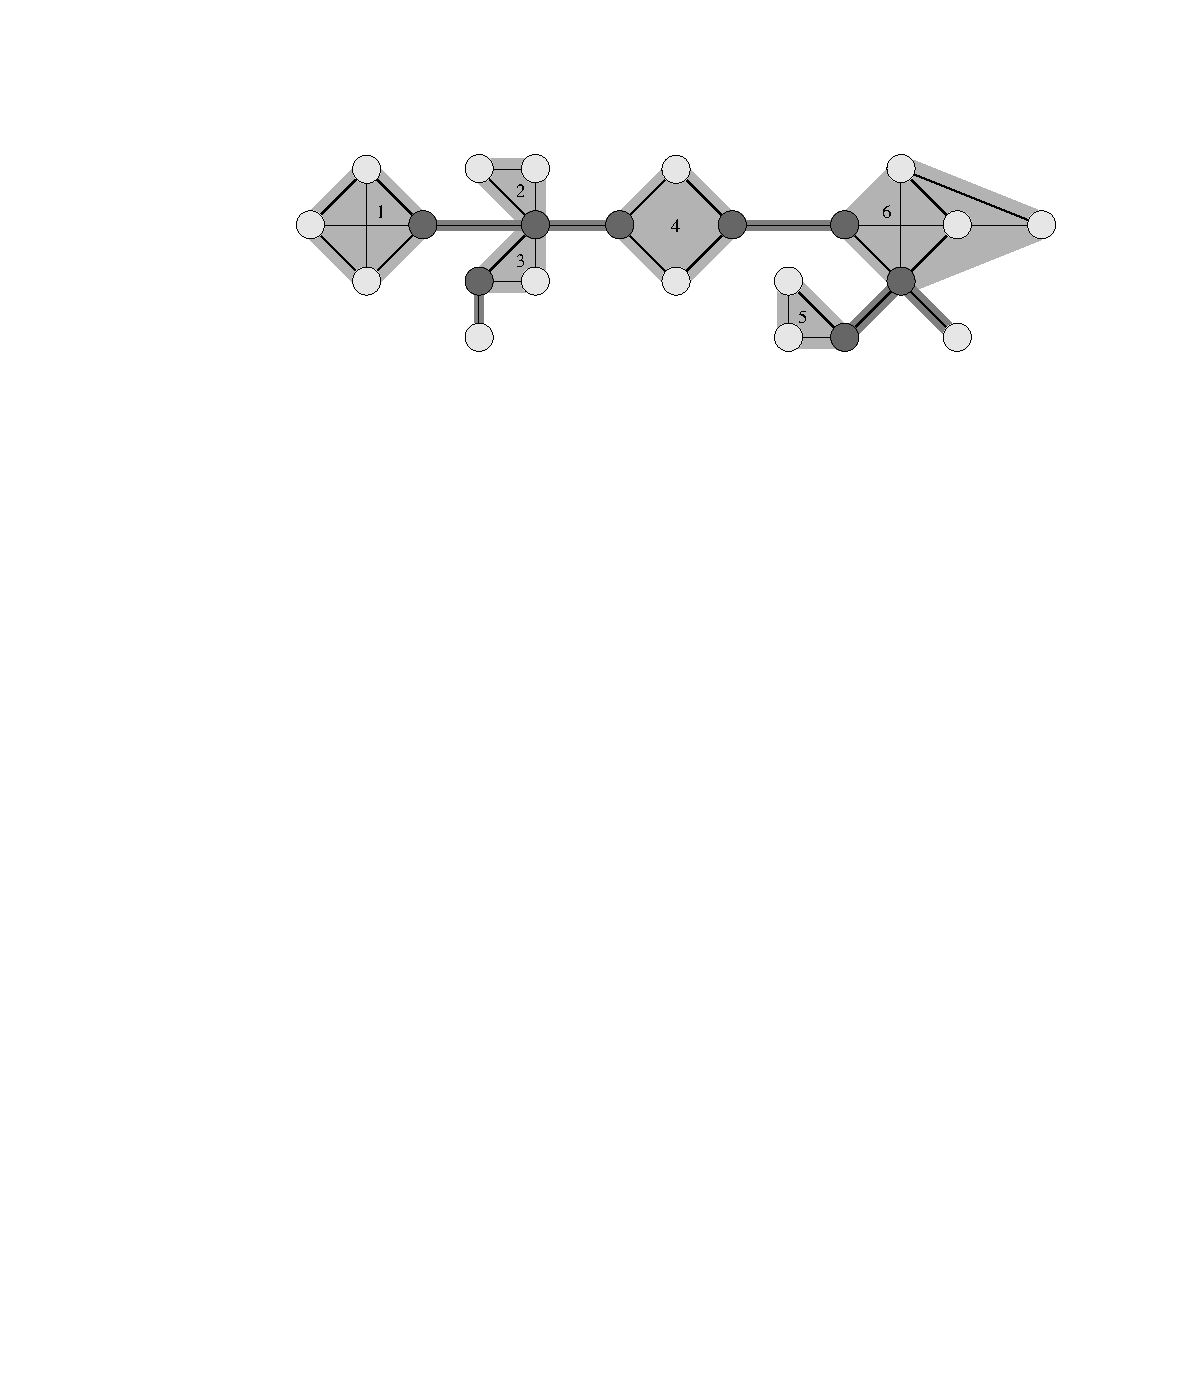
\includegraphics[width=6in]{Fig-Definition.pdf}
	\caption{The definition of articulation points, bridges, and biconnected components. The articulation points are the heavily shaded vertices, the bridges are the heavily shaded edges, and the biconnected components are the edges in the shaded regions, with a \textit{bcc} numbering shown.}
	\label{def}
\end{figure}

~\\
\textbf{Solution.}

\begin{enumerate}
	\item First we let the root be an articulation point and prove it has at least two children.
	
	Assume that the root has less than two children, then after removing this vertex, the other vertices can still remain connected which contradicts to the definition of articulation point. So, the assumption is not right. The root must has at least two children.
	
	Next, we let the root has at least two children and prove it is an articulation point.
	
	When we remove the root, because it has at least two children, the remaining part must be a forest. Every one of its children become a root of the new tree. Then the remaining part is not connected, so the root is an articulation point.
	
	\item 
	First, if an edge lies on a simple cycle, then its removal will not cause the disconnection, because of the property of a cycle. So, we  can say the adverse proposition is also right: if an edge is a brige whose removal cause disconnection, then it doesn't lie on any simple cycle.
	
	Next, if an edge $(u,v)$ dose not lie on any simple cycle. That's to say, we can connect the two vertices $u$ and $v$, only through this edge. Then, if we remove this edge, the vertices $u$ and $v$ must be disconnected. Therefore, the edge is a bridge.
	
	Finally, the proposition is proved.
	
	\item To prove the partition, we need to prove that all nonbridge edges are covered and any two sets have no same edges.
	
	First, from question(b) we can know that if a edge is not a bridge, then it must lies in a cycle. Also,  every maximal simple  cycle corresponds to a biconnected component. Therefore, the biconnected components will cover all of the simple cycles and cover all of the nonbridge edges.
	
	Next, because the biconnected component is a maximal set, if there exists an edge lying on two cycles, then the  two cycle will be merged in to a bigger cycle which can make sure the "maximal". That's to say, there will not be an edge appearing in two biconnected components becausr of the merging.
	
	Finally, the proposition is proved.
\end{enumerate}
	




    \item
    Suppose $G=(V, E)$ is a \textbf{Directed Acyclic Graph} (DAG) with positive weights $w(u, v)$ on each edge. Let $s$ be a vertex of $G$ with no incoming edges and assume that every other node is reachable from $s$ through some path.
    
    \begin{enumerate}
    	\item
    	Give an $O(|V|+|E|)$-time algorithm to compute the shortest paths from $s$ to all the other vertices in $G$. Note that this is faster than Dijkstra's algorithm in general.
    	\item
    	Give an efficient algorithm to compute the longest paths from $s$ to all the other vertices.
    \end{enumerate}
    
    ~\\
       \textbf{Solution.}
       \begin{enumerate}
       	\item To deal with this problem, we can use an algorithm based on  topological sort. 
       	
       	First, We initialize distances to all vertices as infinite and distance of source as 0, then we get a topological sorting array of the graph, which will take $O(|V|+|E|)$ time. 
       	
       Then we traverse the vertices and the edges, and continuously keep the $Dist[i]$ the smallest weight among all previous paths.
       
       Because the vetices have been sorted, so when we traverse and update the smallest weight, it will not affect the previous vetices, which prove the correctness.
       	
       	The detailed algorithm is as follow:
       	
       	\begin{minipage}[t]{0.8\textwidth}
       		\begin{algorithm}[H]
       			\KwIn{DAG $ G=(V,E)$, and a vertex $s  \in V$}
       			\KwOut{Dist[i] which records the shortest paths to the node i}
       			
       			\BlankLine
       			\caption{Shortest Path}\label{Alg_Quick}
       			
       			\ForEach{u $\in$ V}{Dist[u]=$\infty$\;}
       			
       			Dist[s]=0\;
       			
       			Do the topological sort and get a vertices array $Ver$ \;
       			
       			
       			\ForEach {$u \in Ver $}{
       			\ForEach {edge (u,v) $\in$ E }{
       				tmp=Dist[u]+weight(u,v)\;
       				\If{tmp<Dist[v]}{Dist[v]=tmp\;}
       			}	
       				
       				}
       			
       		\end{algorithm}
       	\end{minipage}
       	
       	Then, about the time complexity, line4 (topological sort) takes $O(|V|+|E|)$ time, and line5-line9 is an advanced traversal, which takes $O(|V|+|E|)$. 
       	
       	Therefore, the total time complexity is $O(|V|+|E|)$.
       	
       	
       	\item We can just change the above algorithm littlely to solve this problem. Let  the initial value to be negetive infinite and keep the Dist[i] alway the largest.
       	
       	Obviously  the time complexity is still $O(|V|+|E|)$
       	
       		\begin{minipage}[t]{0.8\textwidth}
       		\begin{algorithm}[H]
       			\KwIn{DAG $ G=(V,E)$, and a vertex $s  \in V$}
       			\KwOut{Dist[i] which records the longest paths to the node i}
       			
       			\BlankLine
       			\caption{Longest Path}\label{Alg_Quick}
       			
       			\ForEach{u $\in$ V}{Dist[u]=$-\infty$\;}
       			
       			Dist[s]=0\;
       			
       			Do the topological sort and get a vertices array $Ver$ \;
       			
       			
       			\ForEach {$u \in Ver $}{
       				\ForEach {edge (u,v) $\in$ E }{
       					tmp=Dist[u]+weight(u,v)\;
       					\If{tmp>Dist[v]}{Dist[v]=tmp\;}
       				}	
       				
       			}
       			
       		\end{algorithm}
       	\end{minipage}
       	
       	
       	
       \end{enumerate}
    
    
    
\end{enumerate}

\vspace{20pt}

\textbf{Remark:} You need to include your .pdf and .tex files in your uploaded .rar or .zip file.

%========================================================================
\end{document}
